\section{Augmented Cube}
In this section, we calculated the full camera matrix in each frame and we used that for projecting a 3D cube into that frame. After that we tried to do the texture mapping on the faces of the cube we projected.

We tried two methods for calculating the projection camera. First method uses chessboard obtained from an arbitrary "first" image, and computes the homography between the first frame and the currently processed frame. It then uses the homography to construct the projection matrix for the camera. The second method uses just the chessboard pattern in the current frame to establish the world origin and relate the camera position towards it.

The second method gives us a better result, probably because the first method computes the homography between two frames and because the frames can have relative distortion with each other and an absolute distortion it will give much worse result.

Now that we found the camera matrix with both methods for testing them we tried to project the chesspattern points in the world coordinate system to the current camera view. All points were projected to the right place in the image so we moved to the next step.
In this step we drew the world coordinate axes attached to the chesspattern plane and then we projected the cube into the current view again attached to the pattern plane.

Last part of this section is texture mapping that we are going to do on the augmented cube. We used five images to mapping on the faces of the cube. For this we mapped each image by using the cube corners and calculating the homography matrix for each face of the cube. We have then used perspective warping to map the texture onto the image where the face should be.

 \begin{figure}[h!]
	\centering
	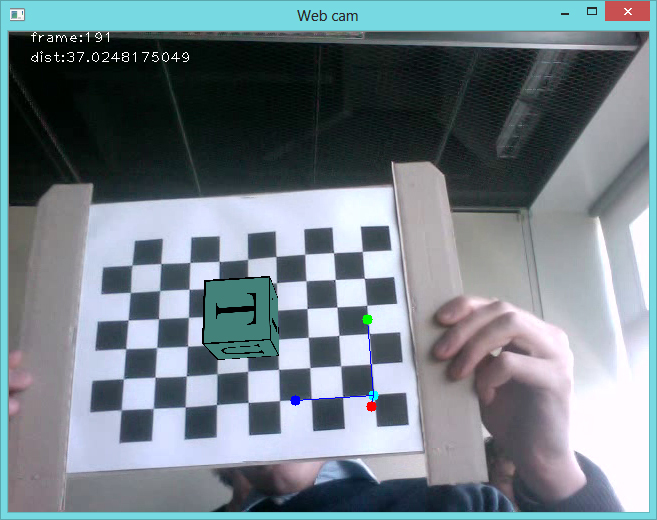
\includegraphics[width=11cm]{Handin3/images/texture.jpg}
	\caption{texture}
	\label{fig:texture}
\end{figure}
